\documentclass[a4paper,twocolumn, 10pt]{article}
\usepackage[p,osf]{scholax}
\usepackage{amsmath,amsthm}
\usepackage[scaled=1.075,ncf,vvarbb]{newtxmath}
\usepackage{graphicx}
\usepackage{mathtools}
\usepackage{float}
\title{This-ness of Elon}
\author{So Okawara}
\begin{document}
\maketitle
\section*{This}
\begin{figure}[H]
\centering
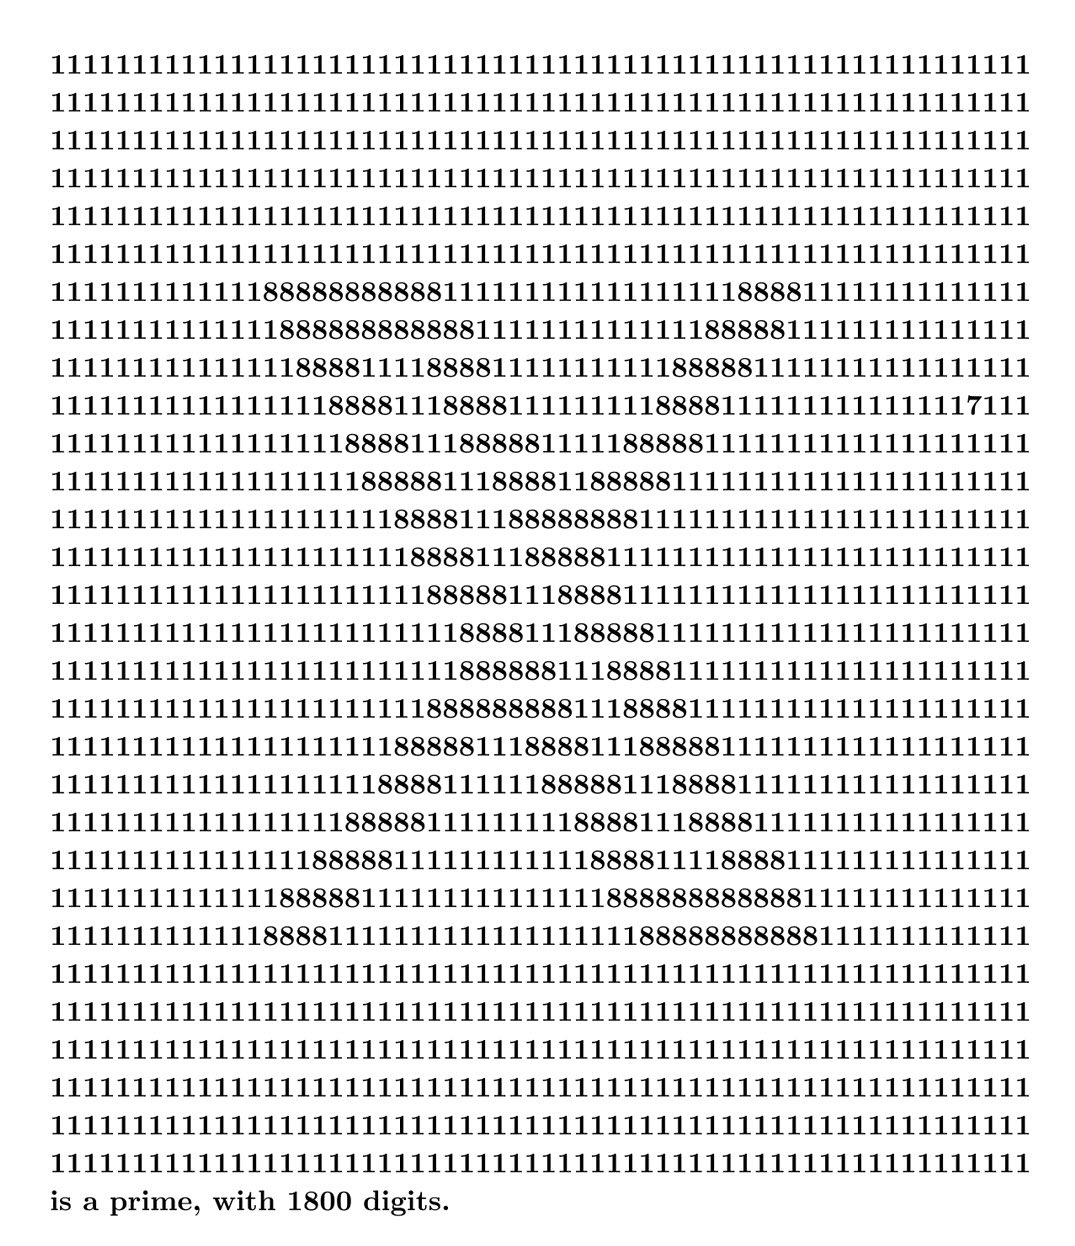
\includegraphics[width=7cm]
{question.png}
\caption{This}
\end{figure}
He says this is a \emph{prime}, and I doubt it. In case, it is, there should be some secret path in math to do this thing, at least semi-systematically. If so, I want to do this in another form. Might this be the problem of \emph{capital}? A metaphysical equivalent of gorgeous vehicle-number or anything? The first critic is the resolution of this image, padding rates, this could be fixed relatively easily; and the second and seriously mathematical point is the selection of $(1,8)$ as the colors to be pixelated. This is openly existing, on $\mathbb{X}$; and I dig it.
\section*{CNN}
However, I'm still a shitpoasting goon in the cave to touch this costly emblem, I should exercise some programming to filtrate only numbers on this .jpg. 
\section*{Prime Painter}
A sort of fresh prince who could write or paint this kind of thing may be on the duty for  $\mathbb{X}$ as a Corp. I adore him/her. A beautiful joking machine for the purity of nothing.
\subsection*{Possible Cost in Theory}
How much resource could one print be costed? How much coud the print be valuable as a picture, or a kind of currency.
\section*{My Work}
This is my print, few, truly high culture for techbros. Good taste, bro.
\section*{What this could be?}
Maybe a true joke since its beauty.
\section*{Penrose Tiling Things \& Its Automation}
This kind of true joke could once in a while emerge in the highly intellectual community where bulky thinking powers are always idling, but what is \emph{this-ness}, this vibe, the brilliant nothing-ness?
\end{document}